% Nature Communications version — reframed around the Allman (2025) critique and
% label-free self-calibration. Base template adapted from main_nature.tex.
% Build: pdflatex + bibtex/biber as per QWEN.md. Figures: Figure_Nature_*.pdf,
% plus new fig3_labelfree.pdf, fig4_prospective.pdf (in ../prl_rewrite_figs/).
\documentclass[11pt]{article}
\usepackage[margin=1in]{geometry}
\usepackage[utf8]{inputenc}
\usepackage[T1]{fontenc}
\usepackage{amsmath,amssymb,bm}
\usepackage{graphicx}
\usepackage{booktabs}
\usepackage{authblk}
\usepackage[colorlinks=true,citecolor=blue,linkcolor=blue,urlcolor=blue]{hyperref}
\usepackage[numbers,sort&compress]{natbib}
\renewcommand\Authfont{\normalsize}
\renewcommand\Affilfont{\footnotesize\itshape}

\title{\textbf{The mutation process label-free calibrates protein language models for viral immune-escape prediction}}

\author[1,2,$\ast$]{Hyoseok Jang}
\author[1,$\ast$]{Sangchul Lee}
\author[3,$\ast$]{David S. Yang}
\author[4]{Haneol Cho}
\author[3,5,$\dagger$]{Cherlhyun Jeong}
\author[1,2,$\dagger$]{Chansoo Kim}
\affil[1]{Computational Science Research Center, Korea Institute of Science and Technology (KIST), Seoul 02792, Republic of Korea}
\affil[2]{AI-Robot Department, University of Science and Technology (UST), Seoul 02792, Republic of Korea}
\affil[3]{Chemical and Biological Integrative Research Center, KIST, Seoul 02792, Republic of Korea}
\affil[4]{Computer Science and Engineering, Sejong University, Seoul 05006, Republic of Korea}
\affil[5]{Division of Bio-Medical Science \& Technology, UST, Seoul 02792, Republic of Korea}
\affil[ ]{\footnotesize $\ast$These authors contributed equally. $\dagger$Correspondence: che.jeong@kist.re.kr, eau@ust.ac.kr}
\date{}

\begin{document}
\maketitle

\begin{abstract}
\noindent
Protein language models (PLMs) are widely used to rank amino-acid substitutions for viral immune escape, but a recent systematic evaluation found that their zero-shot scores fail to separate escape from non-escape mutations and recommended supervised fine-tuning toward specific phenotypes. We show that the missing ingredient is not supervision but the \emph{mutation process}: PLMs score substitutions in protein space, whereas variation is supplied by stochastic nucleotide changes that make some amino-acid substitutions far more accessible than others. We introduce codon-aware constrained semantic change (CAC), a post-hoc calibration that augments any PLM's semantic-change and grammaticality scores with CLIMB, a codon-transition accessibility prior from a continuous-time nucleotide Markov process, requiring no retraining. Crucially, CAC needs no escape labels: freezing the accessibility prior and determining the remaining protein-signal weights by regression against an \emph{independent} phylogenetic-fitness signal---observed-versus-expected substitution counts on the viral tree---recovers the phenotype-supervised weights and matches held-out deep-mutational-scanning escape recovery. The resulting calibration is self-adaptive: it leans on the mutation process when a backbone's protein features are uninformative and on the PLM when they are, without ever seeing escape data. On SARS-CoV-2 Spike, label-free CAC forecasts prospectively, predicting post-cutoff emergent substitutions from pre-cutoff data alone (AUROC $0.90$), and exposes an evolutionary-horizon crossover from mutational accessibility to protein constraint. Coupling the stochastic supply process that generates variants to the protein-level model that scores them thus rescues label-free escape prediction that pure protein-space scoring cannot deliver.
\end{abstract}

\section*{Introduction}

Anticipating how viruses evolve under immune pressure underpins genomic surveillance and vaccine design~\cite{hie2021learning,lin2023evolutionary}. Protein language models (PLMs) enable sequence-based ranking of mutations without explicit structure, casting viral escape as a language problem: viral fitness resembles \emph{grammaticality} and antigenic novelty resembles \emph{semantic change}, and constrained semantic change search (CSCS) prioritizes substitutions that are simultaneously grammatical and semantically large~\cite{hie2021learning}.

This zero-shot framing has, however, been directly challenged. A recent systematic evaluation reported that PLM semantic change does not distinguish escape from non-escape substitutions on SARS-CoV-2 Spike, argued that an undirected embedding shift large enough to ablate antibody binding should equally ablate receptor binding, and concluded that reliable prediction requires \emph{supervised} fine-tuning toward specific phenotypes rather than zero-shot embedding scores~\cite{allman2025systematic}. Recent high-capacity approaches follow exactly this route: CoVFit fine-tunes ESM-2 on surveillance-derived reproduction numbers and deep-mutational-scanning (DMS) escape data to forecast variant fitness~\cite{covfit2025}, and unmodified ESM-2 representations, while informative about evolutionary trajectory~\cite{lamb2026esm}, are typically deployed with task-specific supervision.

We take the opposite view: the zero-shot signal fails not because it lacks labels but because it omits the process that supplies variants. Natural variation is sampled as stochastic nucleotide changes, translated through the genetic code, and only then filtered by selection~\cite{Halpern1998,Rodrigue2010}. Because this genotype-to-phenotype map is uneven, substitutions with comparable PLM scores can differ by orders of magnitude in codon accessibility. Scoring in protein space alone therefore optimizes an objective with a missing feasibility term. The closest prior art, EVEscape, already shows that combining a learned constraint model with an \emph{independent physical prior} (structural accessibility and chemical dissimilarity) yields label-free escape prediction~\cite{thadani2023evescape}; our prior is instead a genotype-level codon-transition Markov process, and---unlike frequency-based fitness inference such as PyR0~\cite{obermeyer2022analysis}---we use the evolutionary signal not to infer fitness but to \emph{calibrate a PLM}.

Here we introduce codon-aware constrained semantic change (CAC): a model-agnostic, post-hoc calibration that augments any PLM's semantic-change and grammaticality scores with CLIMB, a codon-transition accessibility term (Fig.~\ref{fig:1}). We make three contributions. (1) CAC rescues zero-shot escape ranking across PLM backbones, including general-purpose ESM-2 models, without retraining. (2) The calibration is \emph{label-free}: freezing the accessibility prior and determining the two protein-signal weights by regression against an independent phylogenetic-fitness signal---Bloom--Neher observed-versus-expected substitution counts on the SARS-CoV-2 tree~\cite{bloom2023fitness}, which are DMS-independent---recovers the escape-supervised weights and matches held-out DMS recovery. The calibration is self-adaptive, relying on the mutation process when protein features are uninformative and on the PLM when they are. (3) Label-free CAC forecasts prospectively from pre-cutoff data and exposes an interpretable evolutionary-horizon crossover. Together these results answer the label-free-failure critique~\cite{allman2025systematic} without any escape labels.

\begin{figure}[t]
   \centering
   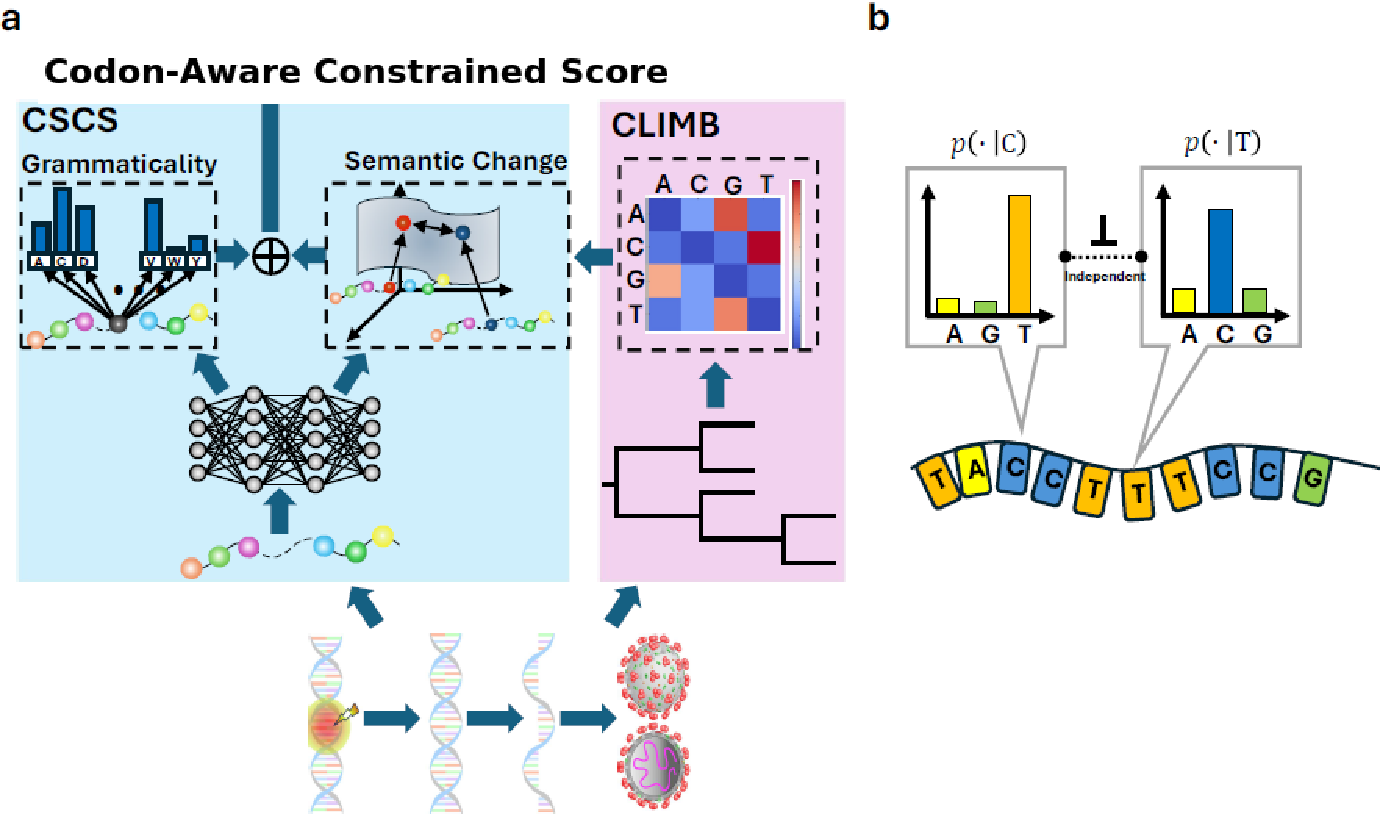
\includegraphics[width=\linewidth]{Figure_Nature_1_revised.pdf}
   \caption{\textbf{Codon-aware, label-free calibration of protein language models.}
   (\textbf{a}) A PLM scores a candidate substitution by semantic change $s_{\rm s}$ (embedding distance) and grammaticality $s_{\rm g}$. CAC adds a codon-accessibility term $s_{\rm p}=\log p_T$ from a continuous-time nucleotide Markov process with generator $\bm{Q}$ estimated from substitution spectra and projected through the genetic code. The three standardized terms are combined; the protein-signal weights are fixed \emph{without escape labels} by regression against an independent phylogenetic-fitness signal.
   (\textbf{b}) Nucleotide biases are non-uniform (e.g. high C$\to$U), so the genetic code maps them to unequal amino-acid accessibilities.}
  \label{fig:1}
\end{figure}

\section*{Results}

\subsection*{A codon-transition prior rescues escape ranking across PLM backbones}

We evaluated all $24{,}187$ nonsynonymous single-nucleotide substitutions of SARS-CoV-2 Wuhan-Hu-1 Spike. Protein scores came from the specialized Hie-BiLSTM model~\cite{hie2021learning}, general-purpose ESM-2 (150M/650M/3B)~\cite{lin2023evolutionary}, and the domain-adapted ESM-2$_{\rm cov}$ (ESM-2-650M further trained on coronaviral sequences; the backbone of CoVFit~\cite{covfit2025}). Validation used published DMS antibody-escape measurements~\cite{baum2020antibody} and characteristic substitutions of major lineages; performance is the mean rank of these annotations (lower is earlier recovery).

Adding the codon-transition prior improved retrospective ranking across backbones and validation sets (Fig.~\ref{fig:2}, Table~\ref{tab:cac_vs_cscs}). On DMS, CAC reduced the ESM-2-3B mean rank from $9130\pm6500$ to $5037\pm3586$ (mean$\pm$s.d.; one-sided Wilcoxon signed-rank $p=3.1\times10^{-3}$), a $44\%$ improvement, with comparable gains for ESM-2-150M ($9387\to5098$) and ESM-2-650M ($8562\to5143$). The specialized Hie-BiLSTM, which already encodes short-horizon substitution structure, changed least ($3757\to3493$, $p=0.55$). A CLIMB-only ablation---ranking by the mutation-process term while the protein scores are randomized---reached a DMS mean rank of $5100\pm184$ across 100 trials, far below the random baseline ($12012\pm1588$) and near the CSCS Hie-BiLSTM baseline. Thus benchmark annotations carry strong genotype-space structure that pure protein-space scoring omits, directly explaining the reported zero-shot failure~\cite{allman2025systematic}: the escape signal that semantic change alone misses is largely the mutation-accessibility signal.

\begin{figure}[t]
    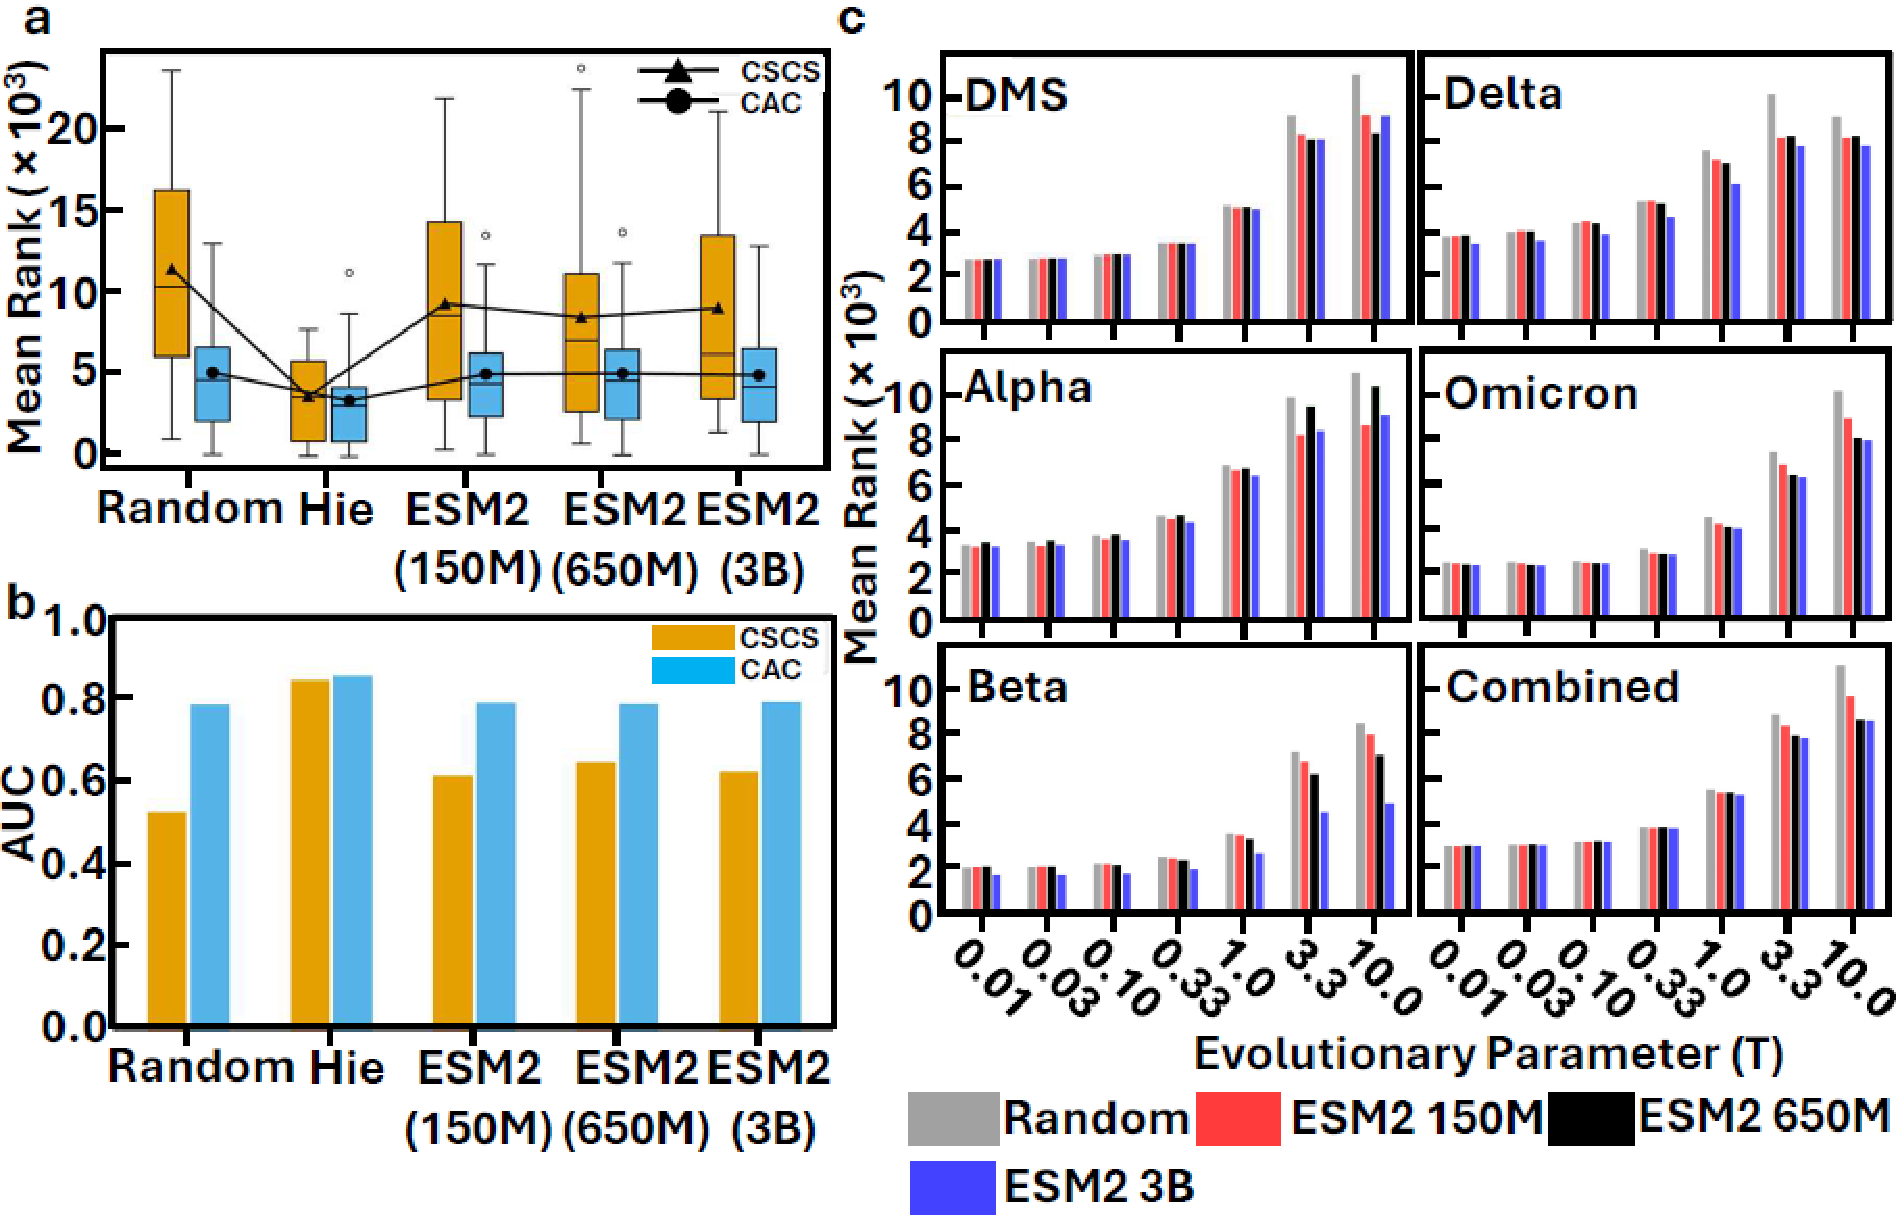
\includegraphics[width=\linewidth]{Figure_Nature_2.pdf}
    \caption{\textbf{Codon-transition calibration improves escape ranking.}
    CAC (green) versus the CSCS baseline (blue), a CLIMB-only ablation, and a random baseline. (\textbf{a}) DMS rank distributions. (\textbf{b}) AUC across backbones. (\textbf{c}) Mean rank versus evolutionary horizon $T$.}
    \label{fig:2}
\end{figure}

\begin{table}[t]
    \centering
    \caption{\textbf{Escape mean ranks (CSCS vs CAC, $T=1$).} One-sided Wilcoxon signed-rank $p$. See Supplementary Table~S1.}
    \begin{tabular}{llccc}
        \toprule
        Set & Backbone & CSCS & CAC & $p$ \\
        \midrule
        DMS & Hie-BiLSTM & $3757\pm2574$ & $3493\pm2974$ & $0.55$ \\
        DMS & ESM-2-150M & $9387\pm6127$ & $5098\pm3667$ & $6.2\times10^{-3}$ \\
        DMS & ESM-2-650M & $8562\pm6870$ & $5143\pm3701$ & $1.3\times10^{-2}$ \\
        DMS & ESM-2-3B & $9130\pm6500$ & $5037\pm3586$ & $3.1\times10^{-3}$ \\
        \midrule
        Combined & Hie-BiLSTM & $6260\pm5378$ & $3841\pm4184$ & $2.4\times10^{-4}$ \\
        Combined & ESM-2-3B & $8736\pm6095$ & $5204\pm4054$ & $8.6\times10^{-6}$ \\
        \bottomrule
    \end{tabular}
    \label{tab:cac_vs_cscs}
\end{table}

\subsection*{The mutation process fixes the calibration without escape labels}

The calibration so far leaves open how to weight the three terms. Choosing them to minimize the escape mean rank on the benchmark is a circular in-sample fit. We instead ask whether the weights can be set from an \emph{independent} evolutionary observable, with no escape labels.

We reparameterize the score by freezing the accessibility prior at unit coefficient (an \emph{offset}) and learning only the two protein-signal weights $(b_0,b_1)$ on semantic change and grammaticality,
\begin{equation}
S \;=\; b_0\,z(s_{\rm s}) + b_1\,z(\log s_{\rm g}) + 1\cdot z(\log p_T).
\label{eq:offset}
\end{equation}
We then fit $(b_0,b_1)$ by regression against per-mutation \emph{phylogenetic fitness}, $\Delta f=\ln[(n_{\rm actual}{+}P)/(n_{\rm expected}{+}P)]$, where expected counts follow the neutral mutation spectrum at four-fold-degenerate sites on the viral tree~\cite{bloom2023fitness}. This signal is DMS-independent (it derives from natural sequence counts, not experiments) and correlates with Spike DMS about as well as two DMS assays correlate with each other, making it a principled, label-free calibration target.

On the domain-adapted ESM-2$_{\rm cov}$ backbone, the label-free weights $(b_0,b_1)=(0.285,0.942)$ closely match the escape-supervised weights $(0.268,0.955)$ obtained by fitting the same form to DMS labels (Fig.~\ref{fig:3}a), and three independent evolutionary signals---all-time substitution frequency, phylogenetic fitness, and an early-period temporal split---converge on the same operating point (Fig.~\ref{fig:3}b). On held-out DMS escape, label-free CAC matches the supervised model (AUROC $0.90$ vs $0.90$; Fig.~\ref{fig:3}c).

The calibration is \emph{self-adaptive}. For general-purpose ESM-2, whose raw protein features carry little escape-specific signal (protein-only AUROC $\approx0.50$), the label-free fit correctly drives the protein weights toward zero and the score falls back on the mutation-process term (CLIB-only AUROC $\approx0.88$), causing no harm. For the domain-adapted ESM-2$_{\rm cov}$, whose features do carry escape information (protein-only AUROC $0.82$), the same procedure recovers the full escape-supervised mixture. In both regimes the independent phylogenetic signal---not any escape label---sets how much the PLM should be trusted.

\begin{figure}[t]
    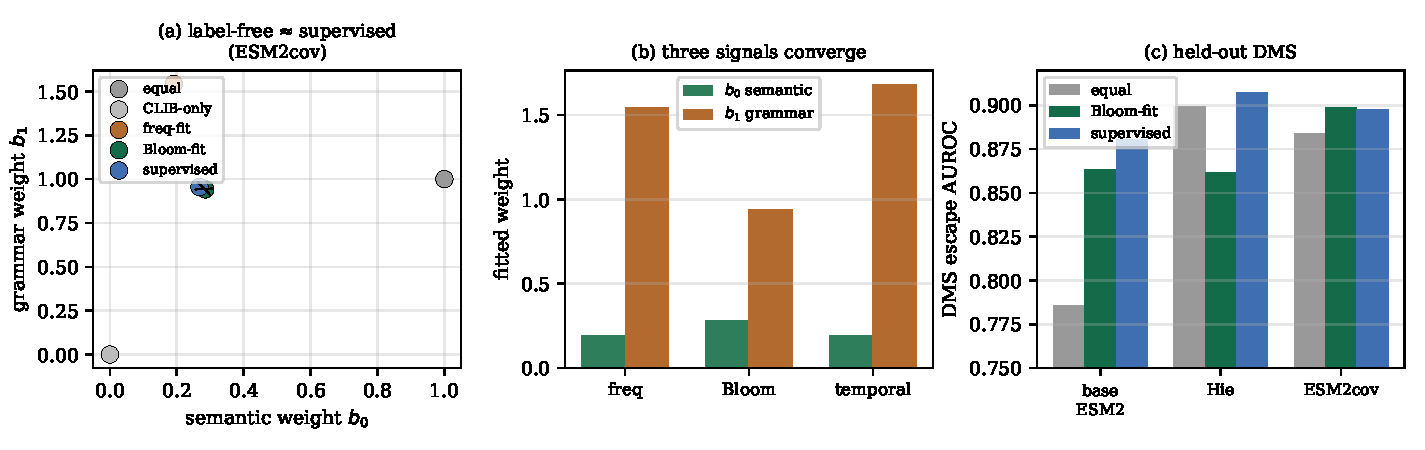
\includegraphics[width=\linewidth]{fig3_labelfree.pdf}
    \caption{\textbf{The mutation process fixes the calibration without escape labels.}
    (\textbf{a}) Label-free weights fit to phylogenetic fitness recover the DMS-supervised weights (ESM-2$_{\rm cov}$). (\textbf{b}) Three independent evolutionary signals (frequency, phylogenetic fitness, temporal split) converge on the same weights. (\textbf{c}) Held-out DMS escape AUROC: label-free matches supervised; for general-purpose ESM-2, whose features are uninformative, the calibration harmlessly reduces to the mutation-process term.}
    \label{fig:3}
\end{figure}

\subsection*{Label-free calibration forecasts prospectively}

A calibration set without escape labels can be made strictly prospective. We fit $(b_0,b_1)$ on substitution frequencies observed \emph{before} a date cutoff and asked whether the resulting score ranks the substitutions that became prevalent \emph{after} the cutoff---a genuine held-out forecast, since the future is unavailable at fit time and the PLM features are frequency-independent.

Across three cutoffs, the pre-cutoff label-free score forecast post-cutoff emergent substitutions at AUROC up to $0.90$ (Fig.~\ref{fig:4}a), significantly above an equal-weight baseline (paired bootstrap $95\%$ CI excludes zero at the two earlier cutoffs; Fig.~\ref{fig:4}b) and on par with the escape-supervised weights ($0.894$), which the label-free fit never sees. Leave-one-variant-out calibration---removing a variant's own defining substitutions before fitting---preserved the improvement on all tested variants, confirming that the gain is not memorization of the evaluated annotations. This directly addresses the prospective-evaluation gap that retrospective benchmarks leave open.

\begin{figure}[t]
    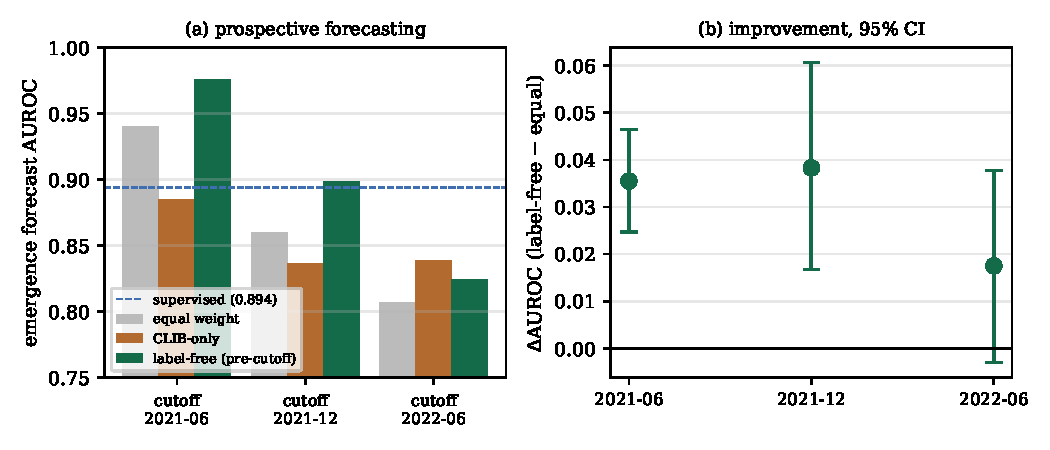
\includegraphics[width=\linewidth]{fig4_prospective.pdf}
    \caption{\textbf{Prospective forecasting without escape labels.}
    (\textbf{a}) Weights fit on pre-cutoff frequency forecast post-cutoff emergent substitutions (AUROC), versus equal-weight, CLIB-only, and the escape-supervised reference. (\textbf{b}) Improvement over equal weight with paired-bootstrap $95\%$ CIs.}
    \label{fig:4}
\end{figure}

\subsection*{An evolutionary-horizon crossover separates supply from constraint}

The Markov horizon $T$ controls how sharply the accessibility prior favors local codon changes. Sweeping $T$ and, for reference, re-optimizing the simplex weights revealed a systematic crossover (Fig.~\ref{fig:2}c and Supplementary): at small $T$ the accessibility term dominates (for Hie-BiLSTM on DMS the optimal CLIMB weight falls from $\gamma=0.54$ at $T=0.1$ to $0.07$ at $T=3$), while at larger $T$ the semantic and grammatical terms carry more weight. Physically, local neighborhoods are bottlenecked by the nucleotide process, whereas broader neighborhoods admit more codon paths and become limited by protein-level compatibility. CAC exposes this supply-versus-constraint tradeoff as an explicit, auditable weight rather than burying it in a black-box predictor.

\section*{Discussion}

A recent systematic evaluation concluded that zero-shot PLM escape scores fail and must be replaced by supervised fine-tuning~\cite{allman2025systematic}. Our results reframe that conclusion: the zero-shot signal is incomplete rather than wrong, and the missing component is the mutation process, not labels. Adding a codon-transition accessibility prior recovers most of the escape signal that semantic change alone misses, and the weighting of protein versus process terms can be fixed by an independent phylogenetic-fitness observable without any escape data. In this sense the stochastic process that \emph{supplies} variants also \emph{calibrates} the model that scores them---a mutation-supply-times-selection decomposition with population-genetic precedent~\cite{Rodrigue2010}, made operational as a plug-in for frozen foundation models.

This label-free calibration differs from the closest alternatives in a specific way. EVEscape couples a learned constraint model to an independent \emph{structural/biophysical} prior~\cite{thadani2023evescape}; our prior is a genotype-level codon-transition process, and we use the independent signal to set the protein/process mixture rather than as a multiplicative factor. CoVFit couples a PLM to an evolutionary-fitness signal but through heavy supervision on surveillance reproduction numbers and DMS escape~\cite{covfit2025}; we use a related evolutionary signal with no escape labels and no fine-tuning. PyR0 infers per-mutation fitness from lineage frequencies~\cite{obermeyer2022analysis}; we do not infer fitness but use such signals to calibrate a protein model. The self-adaptive behavior---down-weighting uninformative PLM features and recovering the supervised mixture for a domain-adapted backbone---emerges because the calibration target is external to both the PLM and the escape benchmark.

Limitations bound these claims. The calibration recovers the supervised mixture only when the backbone carries escape-relevant protein signal, which for SARS-CoV-2 comes from domain adaptation rather than model scale; for general-purpose PLMs the procedure is safe but reduces to the mutation-process term. The accessibility prior is estimated from a context-averaged, single-lineage substitution spectrum and assumes independent sites; context-dependent, lineage-stratified, and path-based extensions are natural. Our evaluation targets single substitutions on one virus; the mechanistic prior is strongest in this regime and, for highly diverged proteins where escape is combinatorial, reduces toward a genetic-distance term, so multi-step and cross-species generalization remain open. Finally, the analysis is a retrospective and prospective ranking study on public data, not an operational forecast or a recommendation to construct variants.

Overall, coupling a mechanistic nucleotide-supply prior to protein-level PLM scores rescues label-free viral-escape ranking, fixes the calibration from an independent evolutionary observable, forecasts prospectively, and renders the supply-versus-constraint tradeoff explicit---turning a reported failure of zero-shot protein-space scoring into a calibration problem solved by the mutation process itself.

\section*{Methods}

\subsection*{CSCS scores}
For sequence $\mathbf{a}\in\mathcal{A}^N$ and substitution $a_i\to\tilde a_i$, semantic change is $s_{\rm s}=d(\mathbf{z},\mathbf{z}[\tilde a_i])$ between sequence embeddings ($\ell^1$ for Hie-BiLSTM, cosine for ESM-2), and grammaticality is $s_{\rm g}=p(\tilde a_i\mid \mathbf{z}_i)$ from the model's positional softmax~\cite{hie2021learning}.

\subsection*{Codon-transition accessibility prior (CLIMB)}
Nucleotides evolve by a continuous-time Markov process on $\mathcal{B}=\{\mathsf A,\mathsf C,\mathsf G,\mathsf U\}$ with generator $\bm Q$; base transitions over horizon $T$ are $[\exp(T\bm Q)]_{uv}$. With independent codon positions, the probability that wild-type codon $\mathbf c$ yields amino acid $\tilde a_i$ is $p_T(\tilde a_i\mid\mathbf c)=\sum_{\tilde{\mathbf c}:g(\tilde{\mathbf c})=\tilde a_i}\prod_{k=1}^3[\exp(T\bm Q)]_{c_k\tilde c_k}$. We estimate $\bm Q$ from SARS-CoV-2 single-base-substitution spectra~\cite{Yi2021Mutational} via $\hat q_{uv}=\hat f_{uv}/\hat\pi_u$ with counts normalized so the mean substitution rate is unity (Supplementary~S1).

\subsection*{CAC score and label-free calibration}
The score is $S=b_0\,z(s_{\rm s})+b_1\,z(\log s_{\rm g})+\kappa\,z(\log p_T)$, with $z(\cdot)$ standardized over all nonsynonymous single-nucleotide substitutions of the reference. Setting $\kappa=0$ recovers CSCS; the simplex form $\alpha z(s_{\rm s})+\beta z(\log s_{\rm g})+\gamma z(\log p_T)$ ($\alpha+\beta+\gamma=1$) is used for the horizon-weight analysis. For label-free calibration we fix $\kappa=1$ and fit $(b_0,b_1)$ by regression against phylogenetic fitness $\Delta f=\ln[(n_{\rm actual}{+}0.5)/(n_{\rm expected}{+}0.5)]$~\cite{bloom2023fitness}, with no escape labels. Escape-supervised weights (for reference only) fit the same form to DMS labels.

\subsection*{Phylogenetic-fitness target and prospective/LOVO validation}
Per-mutation $\Delta f$ and observed substitution frequencies were taken from public phylogenetic and surveillance resources~\cite{bloom2023fitness}. For the prospective test, $(b_0,b_1)$ were fit on frequencies before a date cutoff and evaluated on substitutions that rose in frequency afterward; leave-one-variant-out calibration removed a variant's defining substitutions before fitting. Confidence intervals used paired bootstrap over the positive set.

\subsection*{Models, datasets, and evaluation}
Backbones: Hie-BiLSTM~\cite{hie2021learning}; ESM-2-150M/650M/3B~\cite{lin2023evolutionary}; ESM-2$_{\rm cov}$~\cite{covfit2025}. Validation: DMS escape (Baum et al.~\cite{baum2020antibody}, 19 substitutions on Wuhan-Hu-1, NC\_045512.2) and lineage-defining sets (Alpha, Beta, Delta, Omicron; Supplementary Table~S1). Performance is the mean rank of validation substitutions among 24,187 candidates and AUC/AUROC; the horizon $T\in\{0.01,\dots,10\}$ was swept, and simplex weights minimizing mean rank were computed for 1,000 values of $T$ (Supplementary). Scores were computed on a single NVIDIA H100 GPU.

\section*{Data and code availability}
Source code: \url{https://github.com/sos440/climb}; archived at \url{https://doi.org/10.5281/zenodo.15744443}. Label-free-calibration code and the phylogenetic-fitness and temporal analyses are in the \texttt{research/climb-labelfree} branch.

\bibliographystyle{unsrtnat}
\bibliography{sn-bibliography}

\end{document}
